\RequirePackage{plautopatch}  % pLaTeX または upLaTeX のとき
%\documentclass[uplatex,dvipdfmx,titlepage,a4j]{jsarticle}% upLaTeX のとき
\documentclass[dvipdfmx,titlepage,a4j]{jsarticle}  % pLaTeX のとき
\usepackage{listings,jvlisting}
\usepackage{amsmath,amssymb}
\usepackage{graphicx}
\usepackage[yen]{okuverb}
\usepackage{r04ec-exp}
\usepackage{here}
\usepackage{ascmac}
\usepackage{fancybox}
\usepackage{fancyvrb}
\usepackage{fancyhdr}
\usepackage{lastpage}
\usepackage{otf}

\fancypagestyle{foot}
{
\fancyhead[L]{}
\fancyhead[R]{}
\fancyhead[C]{トランジスタの増幅回路とR-L-C共振回路}
\fancyfoot[C]{\thepage / \pageref{LastPage}}
\renewcommand\headrulewidth{0.4pt}
}

\numberwithin{equation}{section}

%ここからソースコードの表示に関する設定
\lstset{
  language={C++},
  basicstyle={\ttfamily},
  identifierstyle={\small},
  commentstyle={\smallitshape},
  keywordstyle={\small\bfseries},
  ndkeywordstyle={\small},
  stringstyle={\small\ttfamily},
  frame={tb},
  tabsize={2},
  breaklines=true,
  columns=[l]{fullflexible},
  numbers=left,
  xrightmargin=0zw,
  xleftmargin=3zw,
  numberstyle={\scriptsize},
  stepnumber=1,
  numbersep=1zw,
  lineskip=-0.5ex
}

\renewcommand{\lstlistingname}{リスト}
%ここまでソースコードの表示に関する設定

\title{トランジスタの増幅回路とR-L-C共振回路}
% 学年・番号
\grade{4年42番}%
% 氏名
\author{鷲尾 優作}
% 班(後期は班に分かれて実験をする.そのときは,ここに班番号を記入する.)
\team{A1班}
% 提出日
\date{2022年6月16日}
% 実験日
\expdate{2022年5月26日,6月2日,6月9日}
% 共同実験者
% グループに分かれて実験をするテーマでは,グループメンバーの番号名前を書く.
\coauthor{
  14番 & 小林 拓真\\
  24番 & 関 琉斗\\
  26番 & \UTF{9AD9}橋 尚也
}
%
%記載例:
%\coauthor{%
%  2番 & 新潟 花子\\
%  11番 & 三条 次郎}
%%

\begin{document}
\pagestyle{foot}

\maketitle

\section{背景・目的}
電子制御工学科4年前期(4年42番)のトランジスタの増幅回路とR-L-C共振回路実験について報告する.

半導体を用いて製造される能動素子であるトランジスタは, 「増幅作用」をもつが, 信号を増幅させる際,周辺回路の構成によって増幅特性に変化を生じる.
一方受動素子であるインダクタとキャパシタを用いるR-L-C回路は特定の周波数の信号を生成したり,複雑な信号から特定の周波数の信号だけを抽出するのに使用できる.

このレポートでは等価回路による理論値の算出,
バイポーラトランジスタを用いた増幅回路の実験, R-L-C回路共振回路の動作実験をそれぞれ行い,
理論値と実測値を比較しそれぞれの特性を確認した.

\section{トランジスタの増幅回路とその特性}
今回の実験では,エミッタ増幅回路をトランジスタの周辺回路として用いる.
トランジスタに直流バイアス成分を加え活性領域に動作点を設定し,
コンデンサ$C_1$を介して交流信号を重ねてトランジスタのベース端子に入力,
増幅された交流信号をコレクタ端子に接続されたコンデンサ$C_2$を介して取り出す仕組みである.

図\ref{fig:fig1.jpg}にエミッタ増幅回路を示す.
\begin{figure}[H]
  \centering
  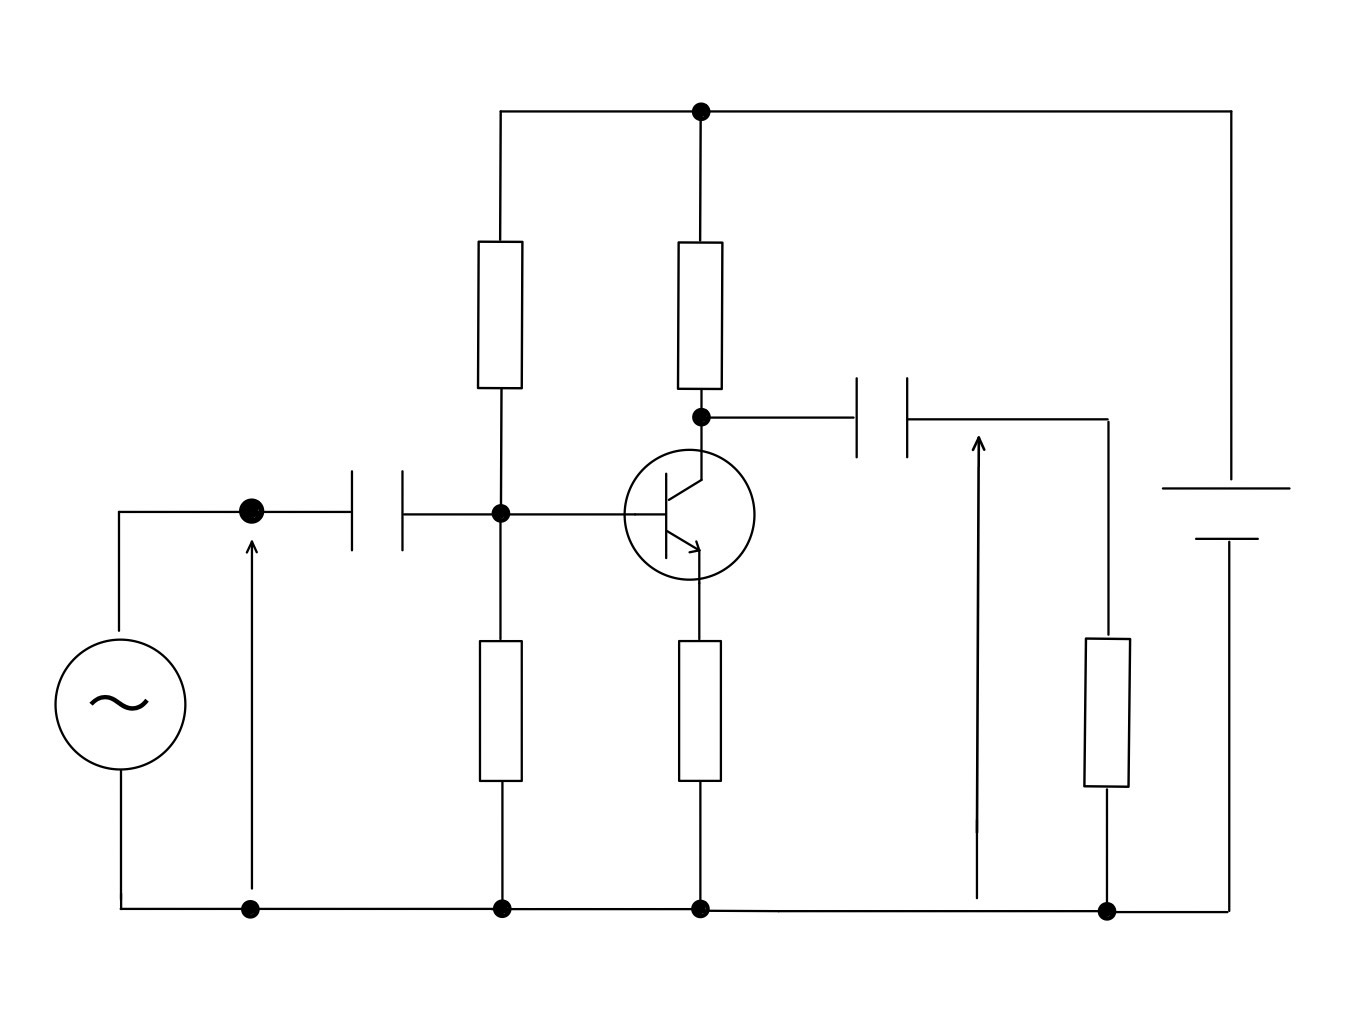
\includegraphics[width=8.5cm]{../fig/fig1.jpg}
  \caption{トランジスタを用いたエミッタ増幅回路}
  \label{fig:fig1.jpg}
\end{figure}

回路図上の各定数は以下のように設定した.\\
$R_1 = 22$ [k$\Omega$], $R_2 = 100$ [k$\Omega$], $R_3 = 2$ [k$\Omega$], $R_4 = 10$ [k$\Omega$], $R_L = 10$ [k$\Omega$]\\
$C_1 = 0.1$ [$\mu$F], $C_2 = 10$ [$\mu$F], $E = 15$ [V]

\subsection{増幅回路の理論特性}
エミッタ増幅回路がどのような特性を示すか推定するため,電気的等価回路を作成し,
代表的な理論値を等価回路から導かれる計算式を用いて計算した.
表\ref{tbl:tr;the}に導出した理論値を記載する.

\begin{table}[htbp]
  \caption{エミッタ増幅回路の各パラメータの理論値}
  \begin{center}
    \begin{tabular}{l|l|r}
      \hline
      各パラメータの詳細    & 名称        & \multicolumn{1}{l}{理論値} \\ \hline \hline
      ベース-GND間電圧      & $V_B$       & 2.7 [V]                    \\ \hline
      コレクタ-GND間電圧    & $V_C$       & 4.5 [V]                    \\ \hline
      エミッタ-GND間電圧    & $V_E$       & 2.1 [V]                    \\ \hline
      ベース-エミッタ間電圧 & $V_{BE}$    & 0.6 [V]                    \\ \hline
      電圧利得              & $G_V$       & 7.8 [dB]                   \\ \hline
      低域カットオフ周波数  & $f_L$       & 93.7 [Hz]                  \\ \hline
      入力インピーダンス    & $\dot{Z}_i$ & 17 [k$\Omega$]             \\ \hline
      出力インピーダンス    & $\dot{Z}_o$ & 10 [k$\Omega$]             \\ \hline
    \end{tabular}
  \end{center}
  \label{tbl:tr;the}
\end{table}

また,各理論値の導出過程については次の通りである.

\subsubsection{バイアス値}
トランジスタにおけるバイアス値は,交流信号を出力する際に基準となる電位の値であり,動作点を決定する重要な
パラメータである.バイアス値を導出する際には回路内の直流分のみを抽出した,「バイアス回路」を考える.

以下図\ref{fig:fig2-bias.jpg}に実験で使用した回路をバイアス回路化したものを示す.
\begin{figure}[H]
  \centering
  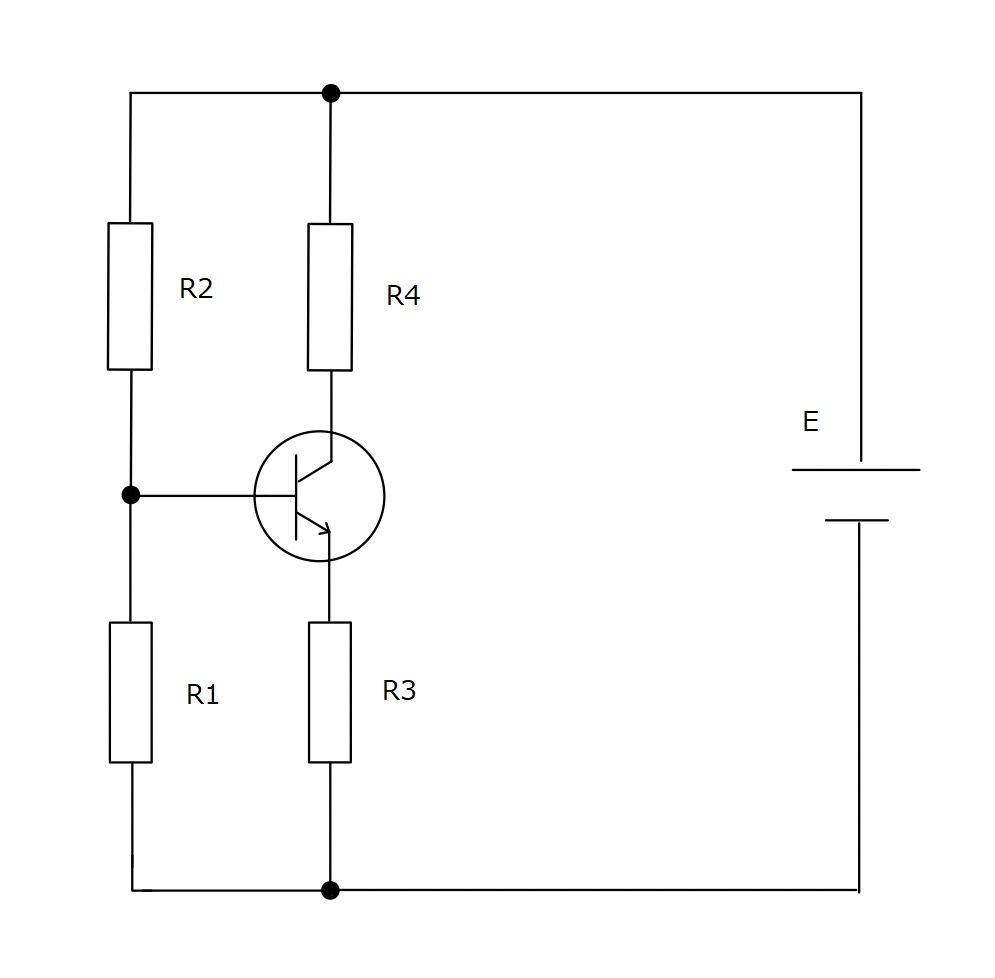
\includegraphics[width=6cm]{../fig/fig2-bias.jpg}
  \caption{エミッタ増幅回路のバイアス回路}
  \label{fig:fig2-bias.jpg}
\end{figure}

まず,ベースGND間電圧$V_B$を導出する.
$I_{R2} \gg  I_B$であると仮定すると,$V_B$の電圧は式(\ref{eq:V_B})のように決定できる.

\begin{equation}
  V_B = \frac{R_1}{R_1 + R_2} \cdot E = \frac{22 \mathrm{[k\Omega]}}{22 \mathrm{[k\Omega]} + 100 \mathrm{[k\Omega]}} \cdot 15 \mathrm{[V]} \approx  2.7 \mathrm{[V]}
  \label{eq:V_B}
\end{equation}

次にエミッタ-GND間電圧$V_{E}$, コレクタ-GND間電圧$V_{C}$を導出する.
動作点を決定するために必要な各電圧$V_{E}$, $V_{C}$を求める計算式は以下のとおりとなる.

\begin{eqnarray}
  V_E &=& V_B - V_{BE} \\
  I_C &=& I_E = \frac{V_E}{R_3} \\
  V_C &=& E - R_4 I_C
\end{eqnarray}

ベース-エミッタ間電圧$V_{BE}$を決定し,各電圧を導く.
使用するバイポーラトランジスタ2SC1815のデータシートより,$I_B - V_{BE}$特性表を図\ref{fig:ibvbe.png}に示す.
\begin{figure}[H]
  \centering
  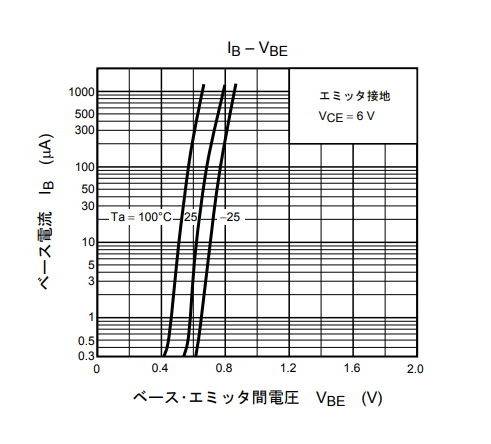
\includegraphics[width=9cm]{../2sc1815/ibvbe.png}
  \caption{2SC1815トランジスタの$I_B$-$V_{BE}$特性}
  \label{fig:ibvbe.png}
\end{figure}

特性表より,$V_{BE}\thickapprox 0.6 \mathrm{[V]}$と読み取ると,代入して各電圧は次のように求められる.
\begin{eqnarray}
  V_E &\approx& 2.7\mathrm{[V]} - 0.6\mathrm{[V]} = 2.1\mathrm{[V]}\\
  \label{eq:I_C}
  I_C &=& \frac{V_E}{R_3} = \frac{2.1\mathrm{[V]}}{2\mathrm{[k\Omega]}} = 1.05\mathrm{[mA]}\\
  V_C &=& E - R_4 I_C = 15\mathrm{[V]} - 10\mathrm{[k\Omega]} \cdot 1.05\mathrm{[mA]} = 4.5\mathrm{[V]}
\end{eqnarray}

\subsubsection{電圧利得}
電圧利得は,入力信号に対して出力信号の比から求められ,入力電圧に対して出力電圧が何[dB]上昇したかを表す.増幅回路そのものの性能を示すうえで重要な
パラメータである.電圧利得を算出するためには,まず結合コンデンサのインピーダンスを0とし,交流分の等価回路を考える.

以下図\ref{fig:fig3-touka.jpg}に実験で使用した回路の結合コンデンサのインピーダンスを0とした交流分の等価回路を示す.

\begin{figure}[H]
  \centering
  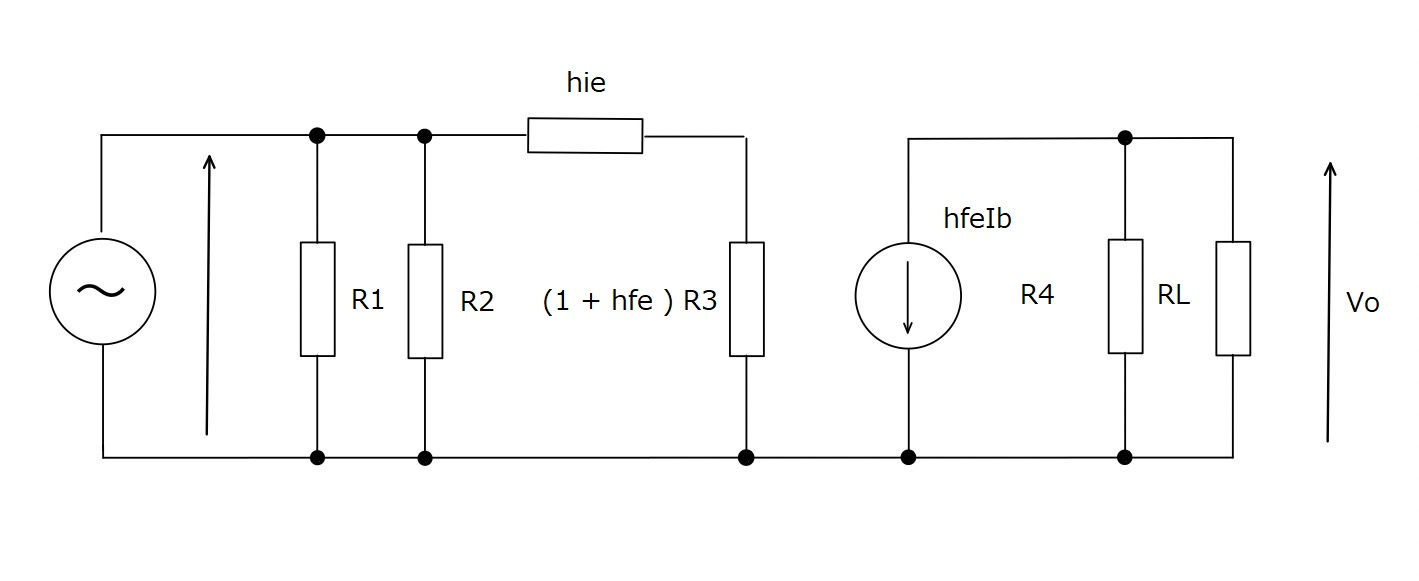
\includegraphics[width=11cm]{../fig/fig3-touka.jpg}
  \caption{エミッタ増幅回路の交流分の等価回路}
  \label{fig:fig3-touka.jpg}
\end{figure}

ここで,入力側の並列抵抗を$R_{12}$,出力側の並列抵抗をを$R_{4L}$のように合成すれば
\begin{eqnarray}
  R_{12} &=& \frac{R_1 R_2}{R_1 + R_2} = \frac{22\mathrm{[k\Omega]} \cdot 100\mathrm{[k\Omega]}}{22\mathrm{[k\Omega]} + 100\mathrm{[k\Omega]}} = 18.0\mathrm{[k\Omega]} \\
  R_{4L} &=& \frac{R_4 R_L}{R_4 + R_L}= \frac{10\mathrm{[k\Omega]} \cdot 10\mathrm{[k\Omega]}}{10\mathrm{[k\Omega]} + 10\mathrm{[k\Omega]}} = 5.0\mathrm{[k\Omega]}
\end{eqnarray}

電圧利得の理論値$G_V$は以下のような式で導出できることがわかる.
\begin{eqnarray}
  V_i &=& h_{ie} I_b + (1+h_{fe})R_3 I_b \\
  V_o &=& h_{fe} I_b R_{4L} \\
  \left\lvert A_v \right\rvert &=& \frac{\left\lvert V_o \right\rvert}{\left\lvert V_i \right\rvert}
  = \frac{h_{fe} R_{4L}}{h_{ie} + (1+h_{fe})R_3} \\
  G_v &=& 20log_{10}(\left\lvert A_v \right\rvert)
\end{eqnarray}

導出に必要な直流電流増幅率$h_{fe}$,トランジスタの入力インピーダンス$h_{ie}$は,データシートより求める.
図\ref{fig:hic.png}に2SC1815のhパラメータ-$I_C$特性表を示す.

\begin{figure}[H]
  \centering
  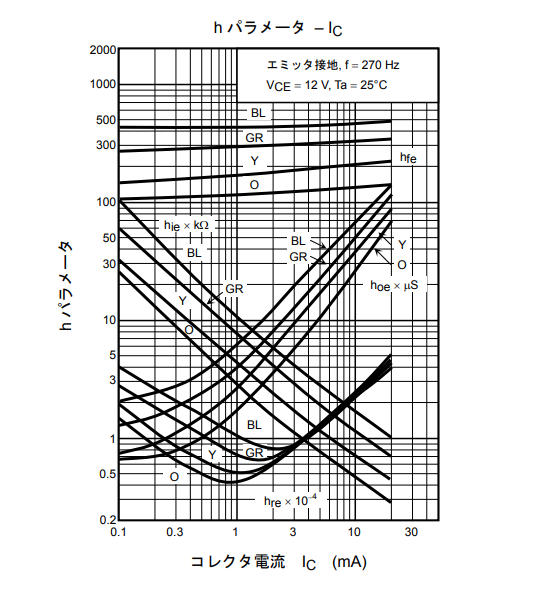
\includegraphics[width=5cm]{../2sc1815/hic.png}
  \caption{2SC1815トランジスタのhパラメータ-$I_C$特性}
  \label{fig:hic.png}
\end{figure}

式(\ref{eq:I_C})より,$I_C \thickapprox 1.0 \mathrm{[mA]}$であるから,
特性表(図\ref{fig:hic.png})より,$h_{fe} \thickapprox 160$,$h_ie \thickapprox 4.0 \mathrm{[k \Omega]}$と読み取れる.

これらの数値を用いて前式を解くと,電圧利得の理論値$G_V$は以下のように導出できる.
\begin{eqnarray}
  V_i &=& 4.0 \mathrm{[k \Omega]} \cdot I_b + (1 + 160) \cdot 10 \mathrm{[k \Omega]} \cdot I_b \thickapprox 2.2\mathrm{[V]}\\
  V_o &=& 4.0 \mathrm{[k \Omega]} \cdot I_b \cdot 5.0\mathrm{[k\Omega]} \thickapprox 5.5\mathrm{[V]}\\
  \left\lvert A_v \right\rvert &=& \frac{\left\lvert V_o \right\rvert}{\left\lvert V_i \right\rvert}
  = \frac{160 \cdot 5.0\mathrm{[k\Omega]}}{4.0 \mathrm{[k \Omega]} + ( 1 + 160 ) \cdot 10 \mathrm{[k \Omega]}} \thickapprox 2.45\mathrm{[倍]}  \\
  G_V &=& 20log_{10}(\left\lvert A_v \right\rvert) \thickapprox 7.8\mathrm{[dB]}
\end{eqnarray}

\subsubsection{低域カットオフ周波数}
低域カットオフ周波数は,入力信号の周波数が減少した際に増幅が正常に行われなくなる現象において,その下限周波数の目安となる
パラメータである.低域カットオフは結合コンデンサ$C_1$によって生じるため,算出するためには結合コンデンサ$C_2$
を無視した簡易等価回路を考える.

以下図\ref{fig:fig4-c2.jpg}に$C_2$を無視した簡易等価回路を示す.
\begin{figure}[H]
  \centering
  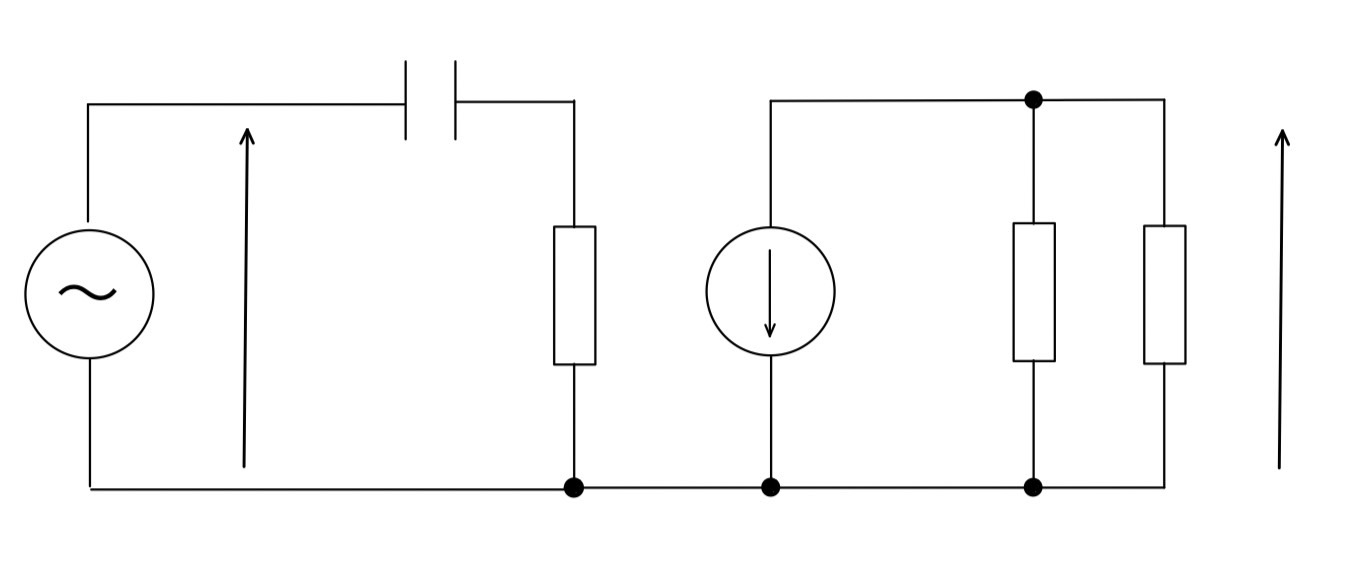
\includegraphics[width=9cm]{../fig/fig4-c2.jpg}
  \caption{$C_2$を無視したエミッタ増幅回路の簡易等価回路}
  \label{fig:fig4-c2.jpg}
\end{figure}

入力電圧を複素数空間に拡張して,
\begin{equation}
  \dot{V} = \dot{V}_{ic} + \dot{V}_{io} = -j \frac{1}{\omega C_1} \dot{I}_i + R_{io} \dot{I}_i
\end{equation}

ここで,各抵抗について
\begin{equation}
  R_{io} = \frac{R_{12} \{h_ie + ( 1 + h_fe)R_3\}}{R_{12} + \{h_ie + ( 1 + h_fe)R_3\}} = \frac{18.0\mathrm{[k\Omega]} \{4.0 \mathrm{[k \Omega]} + ( 1 + 160) 10 \mathrm{[k \Omega]}\}}{18.0\mathrm{[k\Omega]} + \{4.0 \mathrm{[k \Omega]} + ( 1 + 160)10 \mathrm{[k \Omega]}\}} \thickapprox 17 \mathrm{[k \Omega]}
\end{equation}
のように考えれば,

低域カットオフ周波数の定義より,周波数低域において増幅率が最大利得から3[dB]低下する点が$f_L$であるから,
このとき$\dot{V}_{io}$が$\dot{V}_{i}$の$\frac{1}{\sqrt{2}}$倍になることを利用すれば,
$\left\lvert \dot{V}_{ic} \right\rvert = \left\lvert \dot{V}_{io} \right\rvert$が成り立つ.

したがって,低域カットオフ周波数$f_L$は,
\begin{eqnarray}
  \frac{1}{\omega_L C_1} &=& \frac{1}{2 \pi f_L C_1} = R_{io} \\
  f_L &=& \frac{1}{2 \pi C_1 R_{io}} =  \frac{1}{2 \cdot 3.14 \cdot 0.1\mathrm{[\mu F]} \cdot 17 \mathrm{[k \Omega]}} \thickapprox 93.7\mathrm{[Hz]}
\end{eqnarray}

\subsubsection{入力インピーダンス}
回路全体の入力インピーダンスを算出する.
図\ref{fig:fig5-im.jpg}に結合コンデンサ$C_1$,$C_2$のインピーダンスを無視した簡易等価回路を示す.
\begin{figure}[H]
  \centering
  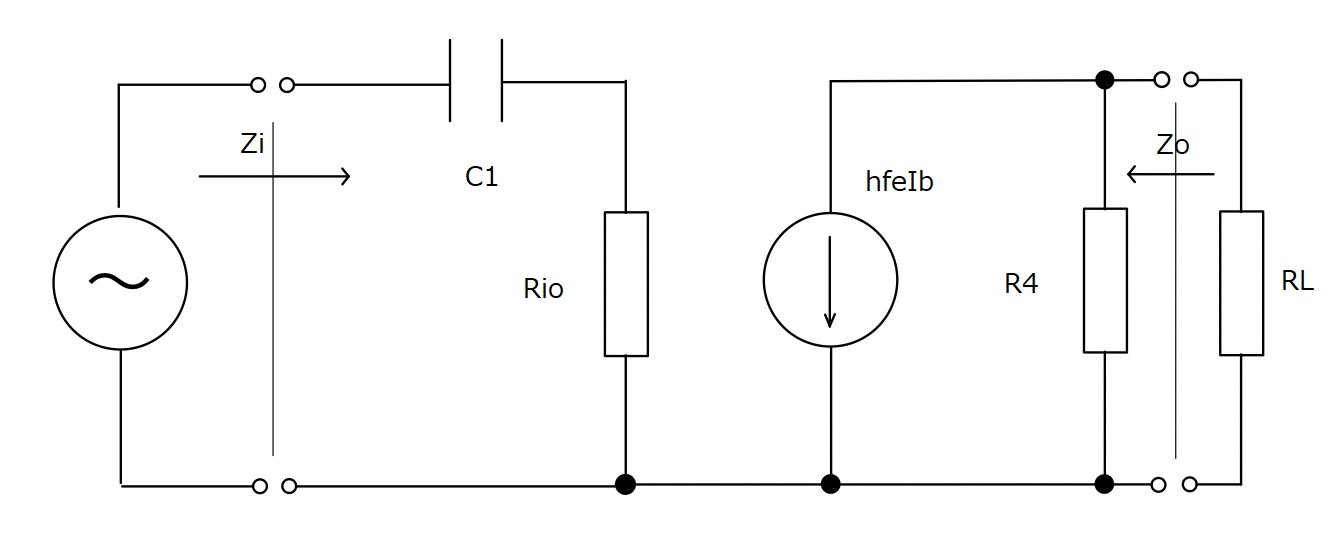
\includegraphics[width=9cm]{../fig/fig5-im.jpg}
  \caption{結合コンデンサのインピーダンスを無視したエミッタ増幅回路の簡易等価回路}
  \label{fig:fig5-im.jpg}
\end{figure}

入力側から見たときの見かけの抵抗が入力インピーダンス$\dot{Z}_i$となるから,
\begin{equation}
  \dot{Z}_i = R_{io} \thickapprox 17 \mathrm{[k \Omega]}
\end{equation}

\subsubsection{出力インピーダンス}
回路全体の出力インピーダンスを算出する.
入力インピーダンスの算出に使用した図\ref{fig:fig5-im.jpg}より

出力側から見たときの見かけの抵抗が出力インピーダンス$\dot{Z}_o$となるから,
\begin{equation}
  \dot{Z}_o = R_4 \thickapprox 10 \mathrm{[k \Omega]}
\end{equation}

\subsubsection{出力波形の歪み}
エミッタ増幅回路では入力信号の電圧$V_i$が一定の条件を満たすとき,正常に増幅されず$V_o$の波形にひずみが生じる.
これには主に2つの原因がある.

\paragraph{ベース電流の遮断}
ベース-エミッタ間電圧$V_{BE}$にかかる直流バイアス成分が十分に大きくない場合,入力信号の電圧$V_i$が小さい場合トランジスタの動作点を下回り
ベース電流$I_B$が遮断されることで,波形がカットされる.

\paragraph{コレクタ電流の飽和}
ベース-エミッタ間電圧$V_{BE}$が大きなとき,トランジスタの動作点が高くなり,コレクタ電流$I_C$が飽和することで出力電圧の波形がカットされる.

\subsection{増幅回路の作成と実測}
図\ref{fig:fig1.jpg}と同様の回路が実装された実験基板を用いて実際に入力を与えその応答を測定する.

表\ref{tbl:tr-list}にエミッタ増幅回路の特性評価に使用した機材のリストを示す.

\begin{table}[H]
  \caption{エミッタ増幅回路の実測機器リスト}
  \centering
  \begin{tabular}{l|l|l|l}
    \hline
    実験装置種別                   & メーカー               & 型番       & 管理番号   \\ \hline\hline
    トランジスタのエミッタ増幅回路 & 長岡高専電子制御工学科 &            & NNCT-EC-03 \\ \hline
    直流安定化電源装置             & 菊水電子工業株式会社   & PMC18-3    & Ec-06      \\ \hline
    低周波発振器                   & GW-INSTEK              & GAG-810    & GEQ874835  \\ \hline
    オシロスコープ                 & GW-INSTEK              & GDS-1052-U & DSO No.11  \\ \hline
    デジタルマルチメータ           & 三和電気計器株式会社   & PC500      & Ec-06      \\ \hline
    デジタルマルチメータ           & 三和電気計器株式会社   & PC500      & Ec-08      \\ \hline
  \end{tabular}
  \label{tbl:tr-list}
\end{table}


図\ref{fig:kiban.jpg}に実験基板の写真を示す.
\begin{figure}[H]
  \centering
  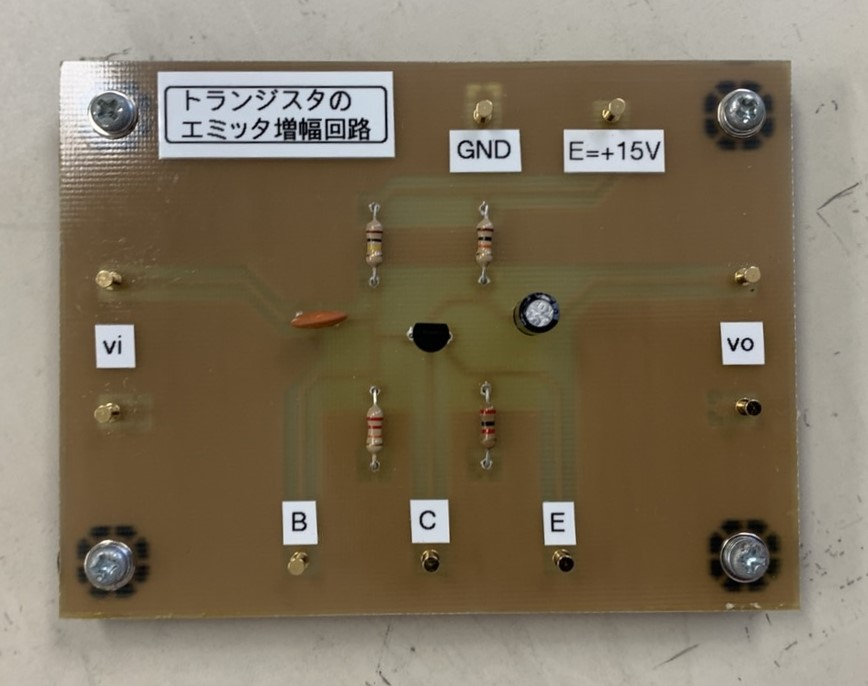
\includegraphics[width=8cm]{../photo/kiban.jpg}
  \caption{トランジスタのエミッタ増幅回路実験基板}
  \label{fig:kiban.jpg}
\end{figure}

実験基板は負荷を可変できるようにするため負荷抵抗$R_L$が取り付けられていないため,$10 \mathrm{[k\Omega]}$の炭素被膜抵抗を$V_0$出力端子部に接続する.

\paragraph{動作確認}
実験基板が正しく動作していることを確認するため,入力電圧と出力電圧をオシロスコープで同時に観測し,反転増幅が発生するかを確認した.
入力信号の周波数は$10 \mathrm{[kHz]}$,最大振幅は$0.4$[$V_{0P}$]とし,得られた波形を図 に示す.

\subsubsection{バイアス電圧の測定}
低周波発振器の出力周波数を0[Hz]に設定し,実験回路内を直流成分のみとし,バイアス電圧を測定する.
測定にはデジタルマルチメータ(直流レンジ)を使用した.

表\ref{tbl:res;bias}にバイアス電圧$V_B$,$V_C$,$V_E$の理論値と実測値をそれぞれ示す.
\begin{table}[H]
  \caption{バイアス電圧の測定結果}
  \begin{center}
    \begin{tabular}{l|l|r|r}
      \hline
      各電圧の位置       & 名称  & \multicolumn{1}{l|}{理論値[$V$]} & \multicolumn{1}{l}{実測値[$V$]} \\ \hline\hline
      ベース-GND間電圧   & $V_B$ & 2.7                              & 2.57                            \\ \hline
      コレクタ-GND間電圧 & $V_C$ & 4.5                              & 5.45                            \\ \hline
      エミッタ-GND間電圧 & $V_E$ & 2.1                              & 1.92                            \\ \hline
    \end{tabular}
  \end{center}
  \label{tbl:res;bias}
\end{table}

\subsubsection{電圧利得の測定}
電圧利得$G_V$は入力電圧$V_i$と出力電圧$V_o$から求められる.
ここでは,デジタルマルチメータ(交流レンジ)によって各電圧の実効値を測定,オシロスコープを使用して最大振幅を測定し,
両者が正しい関係が成り立っていることを確認した上で,電圧利得$G_V$を求めた.

なお,低周波発振器の出力周波数は10[kHz],電圧は0.4[$V_{RMS}$]とする.

表\ref{tbl:res;gain}に入力電圧$V_i$と出力電圧$V_o$の測定結果を示す.
\begin{table}[H]
  \caption{入力電圧と出力電圧の測定結果}
  \begin{center}
    \begin{tabular}{l|l|r|r}
      \hline
      各電圧の位置 & 名称  & \multicolumn{1}{l|}{実効値 [$V_{RMS}$]} & \multicolumn{1}{l}{最大振幅 [$V$]} \\ \hline\hline
      入力電圧     & $V_i$ & 0.402                                   & 0.63                               \\ \hline
      出力電圧     & $V_o$ & 1.024                                   & 1.49                               \\ \hline
    \end{tabular}
  \end{center}
  \label{tbl:res;gain}
\end{table}

\subsubsection{増幅率の周波数特性}
周波数低域において増幅率が最大利得から3[dB]減少する点(低域カットオフ周波数$f_L$)を確認するため,
エミッタ増幅回路の入力電圧$V_i$の周波数$f$を変化させ,増幅率$G_V$の周波数応答を観測する.

低周波発振器の電圧は0.4[$V_{RMS}$]に固定となるよう調整し,出力周波数$f$は10[kHz]から100[kHz]まで適宜変化させた.
このときの周波数に対するデジタルマルチメータ(直流レンジ)で測定した,入力電圧$V_i$,出力電圧$V_o$,またそれらから導出できる電圧利得$G_V$の各値を表\ref{tbl:res;f-gain}に示す.

\begin{table}[H]
  \caption{周波数対増幅率特性の測定結果}
  \begin{center}
    \begin{tabular}{r|r|r|r}
      \hline
      \multicolumn{1}{l|}{入力周波数 $f$ [Hz]} & \multicolumn{1}{l|}{入力電圧 $V_i$ [$V_{RMS}$]} & \multicolumn{1}{l|}{出力電圧 $V_o$ [$V$]} & \multicolumn{1}{l}{電圧利得 $G_V$[dB]} \\ \hline\hline
      10                                       & 0.40                                            & 0.128                                     & -9.897                                 \\ \hline
      20                                       & 0.40                                            & 0.242                                     & -4.365                                 \\ \hline
      50                                       & 0.40                                            & 0.505                                     & 2.025                                  \\ \hline
      70                                       & 0.40                                            & 0.648                                     & 4.190                                  \\ \hline
      80                                       & 0.40                                            & 0.688                                     & 4.711                                  \\ \hline
      90                                       & 0.40                                            & 0.725                                     & 5.166                                  \\ \hline
      95                                       & 0.40                                            & 0.743                                     & 5.379                                  \\ \hline
      100                                      & 0.40                                            & 0.752                                     & 5.483                                  \\ \hline
      110                                      & 0.40                                            & 0.791                                     & 5.922                                  \\ \hline
      120                                      & 0.40                                            & 0.812                                     & 6.150                                  \\ \hline
      130                                      & 0.40                                            & 0.832                                     & 6.361                                  \\ \hline
      170                                      & 0.40                                            & 0.880                                     & 6.848                                  \\ \hline
      200                                      & 0.40                                            & 0.886                                     & 6.907                                  \\ \hline
      220                                      & 0.40                                            & 0.912                                     & 7.159                                  \\ \hline
      270                                      & 0.40                                            & 0.930                                     & 7.328                                  \\ \hline
      320                                      & 0.40                                            & 0.943                                     & 7.449                                  \\ \hline
      500                                      & 0.40                                            & 0.988                                     & 7.854                                  \\ \hline
      1,000                                    & 0.40                                            & 0.994                                     & 7.907                                  \\ \hline
      2,000                                    & 0.40                                            & 0.994                                     & 7.907                                  \\ \hline
      5,000                                    & 0.40                                            & 1.004                                     & 7.993                                  \\ \hline
      10,000                                   & 0.40                                            & 1.038                                     & 8.283                                  \\ \hline
      20,000                                   & 0.40                                            & 1.026                                     & 8.182                                  \\ \hline
      50,000                                   & 0.40                                            & 1.041                                     & 8.308                                  \\ \hline
      100,000                                  & 0.40                                            & 0.902                                     & 7.063                                  \\ \hline
    \end{tabular}
  \end{center}
  \label{tbl:res;f-gain}
\end{table}

表\ref{tbl:res;f-gain}のデータを横軸$f$,縦軸$G_V$として片対数グラフでプロットした.図\ref{fig:f-gv.eps}に示す.

\begin{figure}[H]
  \centering
  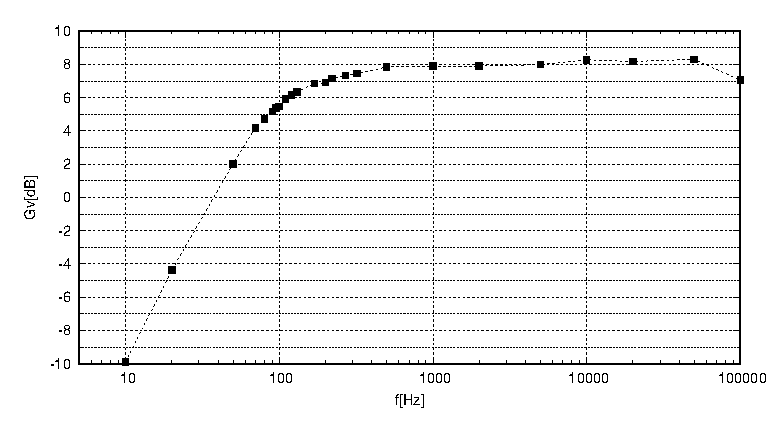
\includegraphics[width=10cm]{../gnuplot/f-gv.eps}
  \caption{周波数対増幅率特性グラフ}
  \label{fig:f-gv.eps}
\end{figure}

\subsubsection{入力インピーダンスの測定}
結合コンデンサ$C_1$と低周波発振器を抵抗$R_R$を介して接続することを考える.
このとき入力インピーダンスは低周波発振器の両端電圧$V_S$,$R_R$の電圧降下後を$V_i$とすれば,式(\ref{eq:Z_I})のように導出できることを利用し,
回路の入力インピーダンスを実測した.

\begin{equation}
  Z_i = \frac{V_i}{V_S - V_i} \cdot R_R
  \label{eq:Z_I}
\end{equation}

低周波発振器の出力周波数を10[kHz],出力電圧を0.4[$V_{RMS}$]とし,デジタルマルチメータ(交流レンジ)で測定した$V_S$,$V_i$の各電圧を表\ref{tbl:res;Z_I}に示す.

\begin{table}[H]
  \caption{負荷抵抗$R_R$による入力インピーダンスの測定結果}
  \begin{center}
    \begin{tabular}{l|l|l}
      \hline
      入力電圧 $V_S$ [$V_{RMS}$] & $R_R$による電圧降下後の電圧 $V_i$ [$V_{RMS}$] & 入力インピーダンス $Z_i$ [$\Omega$] \\ \hline\hline
      \multicolumn{1}{r|}{0.4}   & \multicolumn{1}{r|}{0.254}                    & \multicolumn{1}{r}{17.397}          \\ \hline
    \end{tabular}
  \end{center}
  \label{tbl:res;Z_I}
\end{table}


\subsubsection{出力インピーダンスの測定}
エミッタ増幅回路の出力端子の解放電圧$V_{oo}$に対して,出力端子に負荷抵抗$R_L$を接続した際の$R_L$の両端電圧$V_o$を介して接続することを考える.
このとき出力インピーダンスは式(\ref{eq:Z_O})のように導出できることを利用し,回路の出力インピーダンスを実測した.

\begin{equation}
  Z_o = \frac{V_{oo} - V_o}{V_o} \cdot R_L
  \label{eq:Z_O}
\end{equation}

低周波発振器の出力周波数を10[kHz],出力電圧を0.4[$V_{RMS}$]とし,デジタルマルチメータ(交流レンジ)で測定した$V_{oo}$,$V_o$の各電圧を表\ref{tbl:res;Z_O}に示す.

\begin{table}[H]
  \caption{負荷抵抗$R_L$による出力インピーダンスの測定結果}
  \begin{center}
    \begin{tabular}{l|l|l}
      \hline
      端子間解放電圧 $V_{oo}$ [$V_{RMS}$] & $R_L$接続時の両端電圧 $V_o$ [$V_{RMS}$] & 出力インピーダンス $Z_o$ [$\Omega$] \\ \hline\hline
      \multicolumn{1}{r|}{2.019}          & \multicolumn{1}{r|}{1.019}              & \multicolumn{1}{r}{9.813}           \\ \hline
    \end{tabular}
  \end{center}
  \label{tbl:res;Z_O}
\end{table}

\subsubsection{増幅率の測定と波形歪みの観測}

\section{R-L-C共振回路とその特性}
R-L-C共振回路は,抵抗(Resistance),インダクタ(Inductance),キャパシタ(Capacitance)のそれぞれのインピーダンス特性を
利用し交流信号を入力として共振させることで周波数に対して特殊な応答を生じる回路である.

図\ref{fig:fig6-rcl.jpg}にR-C-L共振回路を示す.
\begin{figure}[H]
  \centering
  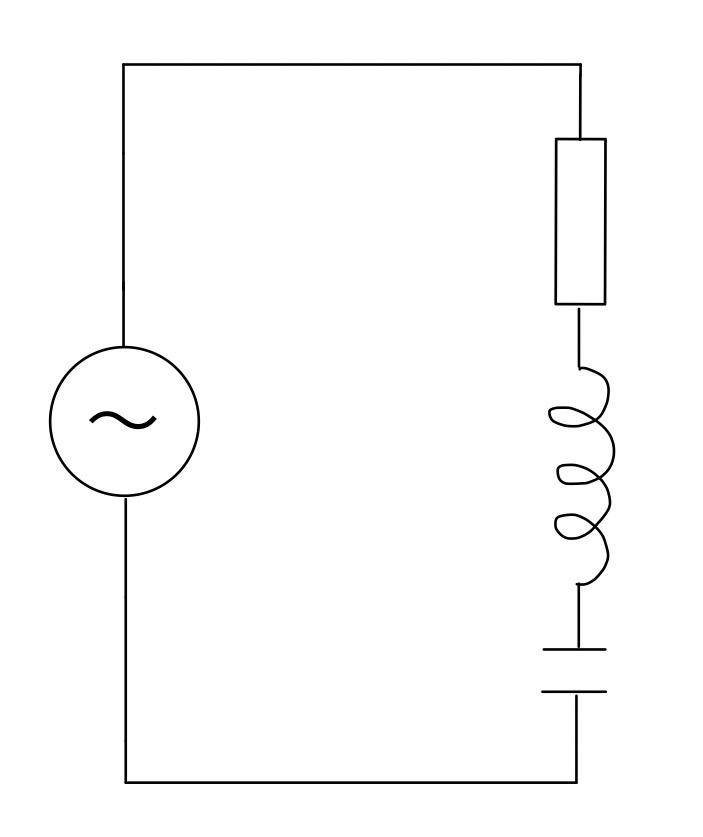
\includegraphics[width=5cm]{../fig/fig6-rcl.jpg}
  \caption{R-L-C共振回路}
  \label{fig:fig6-rcl.jpg}
\end{figure}

R-L-C共振回路は共振によって入力した周波数に対して全体のアドミッタンスが変化するアドミッタンス周波数特性を持つ.
アドミッタンスが最大となる入力周波数を$f_0$,最大値から$\frac{1}{\sqrt{2}}$倍となる周波数を$f_1$,$f_2$とすると.
アドミッタンス周波数特性は図 のようになる.

また,R-L-C共振回路ではアドミタンスの実部と虚部であるコンダクタンスとサセプタンスをXY成分としてプロットすると
円を描くことが知られている.この円を「アドミッタンスループ」と呼び,アドミッタンスループの各特徴点から有用な周波数や回路解析を行うことができる.
図 にアドミタンスループを示す.

\subsection{定数と理論特性}
\subsubsection{アドミッタンスと共振周波数}
図において角周波数$\omega$の信号を入力することを考える.
ここで回路全体のアドミッタンス$Z$は次式のようになるので,

\begin{equation}
  Z = R + j(\omega L - \frac{1}{\omega C})
\end{equation}

この時,複素アドミッタンス$\dot{Y}$とその大きさYは以下の式で求められる.

\begin{eqnarray}
  \dot{Y} &=& \frac{1}{Z} = \frac{1}{R + j(\omega L - \frac{1}{\omega C})} \\
  Y &=& \frac{1}{\dot{Y}} = \frac{1}{\sqrt{R + j(\omega L - \frac{1}{\omega C})}}
\end{eqnarray}

共振時にはアドミッタンスは最大となるから,このときの角共振周波数$\omega_0$,複素アドミッタンスの大きさ$Y_0$とすると,
複素アドミッタンス$\dot{Y}$の分母が最大となる時が$Y_0$であるから,以下のように表せる.

\begin{eqnarray}
  \omega_0 L - \frac{1}{\omega_0 C} &=& 0 \\
  \omega_0 &=& \frac{1}{\sqrt{LC}} \\
  Y_0 &=& \frac{1}{\sqrt{R}}
\end{eqnarray}

\subsubsection{アドミッタンスループ}

複素パラメータ$R$(レジスタンス),$X$(リアクタンス),
$G$(コンダクタンス),$B$(サセプタンス)は複素インピーダンス$\dot{Z}$と次式のような関係を持つ.

\begin{eqnarray}
  \dot{Z} = R + jX \\
  \dot{Y} = G + jB
\end{eqnarray}

2式の関係性を考えると,

\begin{eqnarray}
  R + jX &=& \frac{1}{G + jB} = \frac{G}{G^2 + B^2} -j\frac{B}{G^2 + B^2} \\
  R &=& \frac{G}{G^2 + B^2} \\
  0 &=& G^2 + B^2 - \frac{G}{R}
\end{eqnarray}

ここで,両辺に$(\frac{1}{2R})^2$を加算して式を整理すると,円の方程式が得られる.

\begin{eqnarray}
  (G - \frac{1}{2R})^2 + B^2 &=& (\frac{1}{2R})^2 \\
\end{eqnarray}

したがって,$G$(コンダクタンス),$B$(サセプタンス)を平面上にプロットしたとき描く円の
中心座標は,$(\frac{1}{2R}, 0)$,半径$\frac{1}{2R}$と定まる.

\subsubsection{品質係数Q値の算出}
Q値(Quality Factor)は,共振回路の共振のピークの鋭さを表す指標である.

R-L-C共振回路においては一般的に
\begin{eqnarray}
  Q = \frac{\omega_0 L}{R} = \frac{1}{\omega_0 CR}
\end{eqnarray}

となることが知られている.

これを証明する.
振動の共振ピークの$\sqrt{2}$倍となる入力周波数$\omega_2$,$\omega_1$とすると,
$\omega_2$,$\omega_1$におけるYの大きさは

\begin{eqnarray}
  Y &=& \frac{Y_0}{\sqrt{2}} = \frac{1}{\sqrt{2}R} \\
  Y &=& \frac{1}{\sqrt{R^2 + (\omega L - \frac{1}{\omega C})^2}}
\end{eqnarray}

$R$(レジスタンス)について整理すると

\begin{eqnarray}
  2R^2 &=& R^2 + (\omega L - \frac{1}{\omega C})^2 \\
  \pm R &=& (\omega L - \frac{1}{\omega C})
\end{eqnarray}

両辺に$\omega C$をかけて$\omega$を導くと

\begin{eqnarray}
  LC \omega^2 + RC\omega = 0\\
  \omega = \frac{\pm RC \pm \sqrt{(RC)^2 + 4LC}}{2LC}
\end{eqnarray}

$\omega_2 > \omega_1 > 0$であるから,

\begin{eqnarray}
  \omega_1 &=& \frac{-RC + \sqrt{(RC)^2 + 4LC}}{2LC} \\
  \omega_2 &=& \frac{+RC + \sqrt{(RC)^2 + 4LC}}{2LC} \\
  \omega_2 - \omega_1 &=& \frac{R}{L}
\end{eqnarray}

ここでQ値の定義を考えると

\begin{eqnarray}
  Q &=& \frac{\omega_0 L}{R} = \frac{\omega_0}{\omega2 - \omega_1}\\
\end{eqnarray}

となる.

\subsubsection{R, L, C値の算出方法}
R-L-Cの各定数が不明な際でも,アドミッタンスループを観測し$Y_0$,$\omega_0$,$\omega_1$,$\omega_2$を測定することで,
各定数成分を決定することができる.$R$,$L$,$C$は,それぞれ以下の式のとおり解析できる.

\begin{eqnarray}
  R &=& \frac{1}{Y_0} \\
  L &=& \frac{Q}{\omega_0 Y_0} \\
  C &=& \frac{Y_0}{\omega_0 Q}
\end{eqnarray}

\subsection{R-L-C回路のアドミッタンス特性測定と定数の算出}

\subsubsection{アドミッタンス特性の測定}
R-L-C回路の特性評価を行うことができるLCRメーターを使用して入力周波数を自動で広範囲に可変し,アドミッタンス,
コンダクタンス,サセプタンスを測定することで,回路の周波数特性およびアドミッタンスループの観測を狙う.

図\ref{fig:fig7-meter.jpg}に測定機器の概要を図示する.
\begin{figure}[H]
  \centering
  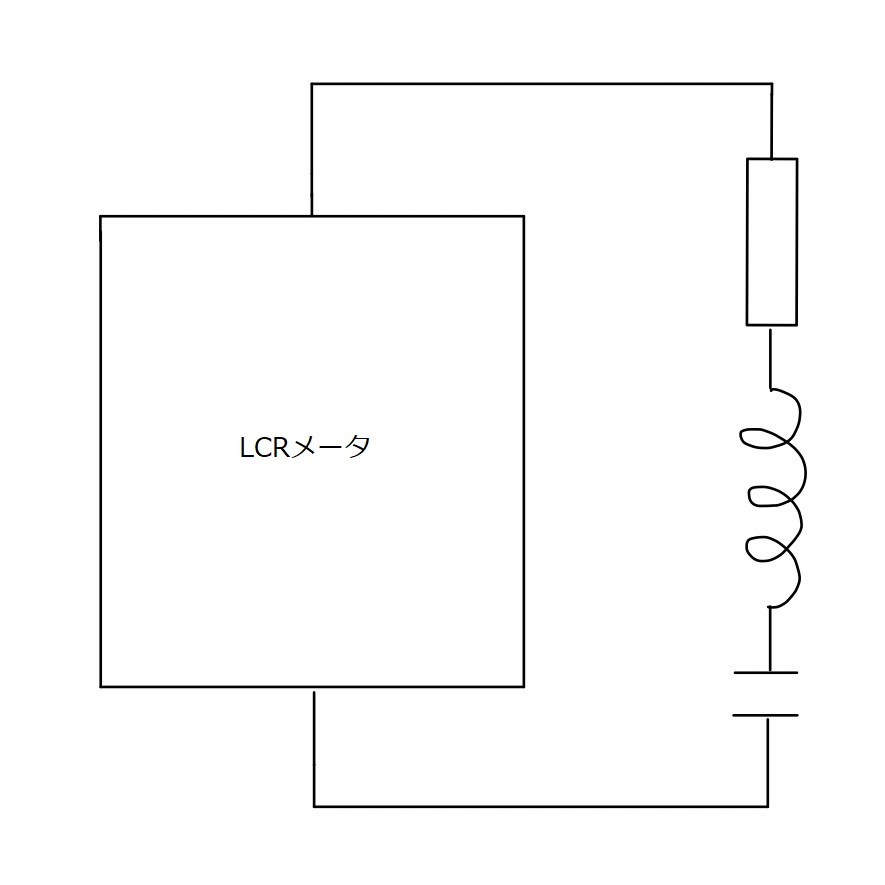
\includegraphics[width=6cm]{../fig/fig7-meter.jpg}
  \caption{LCRメーターを用いたアドミッタンス特性測定の概要}
  \label{fig:fig7-meter.jpg}
\end{figure}

表\ref{tbl:r-l-c-list}にR-C-L共振回路の特性評価に使用した機材を示す.

\begin{table}[htbp]
  \caption{R-L-C共振回路の実測機器リスト}
  \begin{center}
    \begin{tabular}{l|l|l|l}
      \hline
      実験装置種別 & メーカー                 & 型番   & 製造番号         \\ \hline \hline
      LCRメータ    & エヌエフ回路設計ブロック & ZM2375 & BH16H24S00000033 \\ \hline
    \end{tabular}
  \end{center}
  \label{tbl:r-l-c-list}
\end{table}


\paragraph{アドミタンス周波数特性}
LCRメータの掃引周波数を2[kHz]から8[kHz]に設定し,1201[ポ0イント]の測定点において,周波数$f$に対する複素アドミッタンスの大きさ$Y$の変化を観測した.

表\ref{tbl:lcrm-admitance}にLCRメーターの各設定値を示す.

\begin{table}[H]
  \caption{アドミッタンス周波数特性測定時のLCRメータ設定値}
  \begin{center}
    \begin{tabular}{l|l|l|l}
      \hline
      種別           & 分類                          & 項目           & 設定値                       \\ \hline\hline
      表示           & 主パラメタ                    & 種類           & Y                            \\ \hline
      表示           & 主パラメタ                    & 偏差表示       & ABS                          \\ \hline
      測定           & 周波数                        & 周波数         & \multicolumn{1}{r}{1.00E+03} \\ \hline
      測定           & 信号レベル                    & ALC            & OFF                          \\ \hline
      測定           & 信号レベル                    & 測定電圧レベル & \multicolumn{1}{r}{1}        \\ \hline
      測定           & 信号レベル                    & 測定電流レベル & \multicolumn{1}{r}{1.00E-03} \\ \hline
      測定           & レンジ                        & 自動選択       & ON                           \\ \hline
      測定           & レンジ                        & 測定レンジ     & 1kΩ                          \\ \hline
      測定           & トリガ                        & トリガ源       & Internal                     \\ \hline
      測定           & トリガ                        & 遅延時間       & \multicolumn{1}{r}{0.008}    \\ \hline
      測定           & 測定速度                      & 測定速度       & MED                          \\ \hline
      測定           & DCバイアス                    & 有効無効       & OFF                          \\ \hline
      測定           & 平均化                        & 有効無効       & OFF                          \\ \hline
      [スイープ測定] &                               &                &                              \\ \hline
      タイプ         & リニア                        &                &                              \\ \hline
      開始周波数     & \multicolumn{1}{r|}{2.00E+03} &                &                              \\ \hline
      終了周波数     & \multicolumn{1}{r|}{8.00E+03} &                &                              \\ \hline
      測定点数       & \multicolumn{1}{r|}{1201}     &                &                              \\ \hline
    \end{tabular}
  \end{center}
  \label{tbl:lcrm-admitance}
\end{table}

測定値を縦軸に$Y$を横軸に$f$をとりグラフ化した.図\ref{fig:A_YTheta.eps}に示す.
\begin{figure}[H]
  \centering
  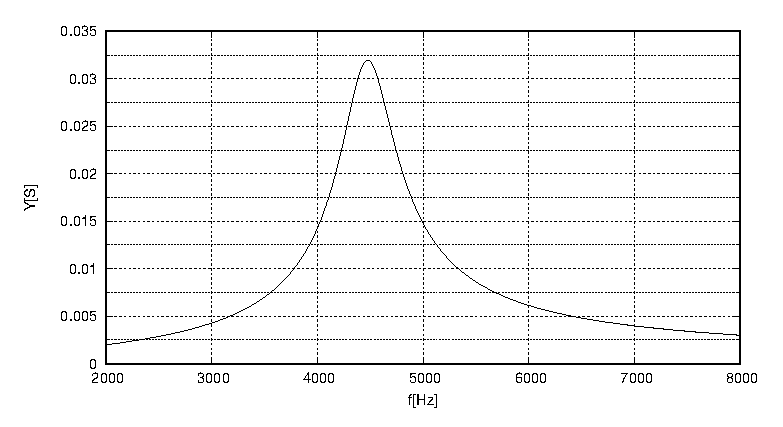
\includegraphics[width=10cm]{../gnuplot/A_YTheta.eps}
  \caption{R-L-C共振回路のアドミッタンス周波数特性}
  \label{fig:A_YTheta.eps}
\end{figure}

\paragraph{アドミッタンスループ特性}
LCRメータの掃引周波数を2[kHz]から8[kHz]に設定し,1201[ポ0イント]の測定点において,周波数$f$に対するコンダクタンス$G$,サセプタンス$B$の変化を観測した.

表\ref{tbl:lcrm-admitance-loop}にLCRメーターの各設定値を示す.
\begin{table}[H]
  \caption{アドミッタンスループ測定時のLCRメータ設定値}
  \begin{center}
    \begin{tabular}{l|l|l|l}
      \hline
      種別           & 分類                          & 項目           & 設定値                       \\ \hline\hline
      表示           & 主パラメタ                    & 種類           & G                            \\ \hline
      表示           & 主パラメタ                    & 偏差表示       & ABS                          \\ \hline
      表示           & 副パラメタ                    & 種類           & B                            \\ \hline
      表示           & 副パラメタ                    & 偏差表示       & ABS                          \\ \hline
      測定           & 周波数                        & 周波数         & \multicolumn{1}{r}{1.00E+03} \\ \hline
      測定           & 信号レベル                    & ALC            & OFF                          \\ \hline
      測定           & 信号レベル                    & 測定電圧レベル & \multicolumn{1}{r}{1}        \\ \hline
      測定           & 信号レベル                    & 測定電流レベル & \multicolumn{1}{r}{1.00E-03} \\ \hline
      測定           & レンジ                        & 自動選択       & ON                           \\ \hline
      測定           & レンジ                        & 測定レンジ     & 1kΩ                          \\ \hline
      測定           & トリガ                        & トリガ源       & Internal                     \\ \hline
      測定           & トリガ                        & 遅延時間       & \multicolumn{1}{r}{0.008}    \\ \hline
      測定           & 測定速度                      & 測定速度       & MED                          \\ \hline
      測定           & DCバイアス                    & 有効無効       & OFF                          \\ \hline
      測定           & 平均化                        & 有効無効       & OFF                          \\ \hline
      [スイープ測定] &                               &                &                              \\ \hline
      タイプ         & リニア                        &                &                              \\ \hline
      開始周波数     & \multicolumn{1}{r|}{2.00E+03} &                &                              \\ \hline
      終了周波数     & \multicolumn{1}{r|}{8.00E+03} &                &                              \\ \hline
      測定点数       & \multicolumn{1}{r|}{1201}     &                &                              \\ \hline
    \end{tabular}
  \end{center}
  \label{tbl:lcrm-admitance-loop}
\end{table}

測定値を縦軸に$B$を横軸に$G$をとり複素数空間にグラフ化した.図\ref{fig:A_GB.eps}に示す.
\begin{figure}[H]
  \centering
  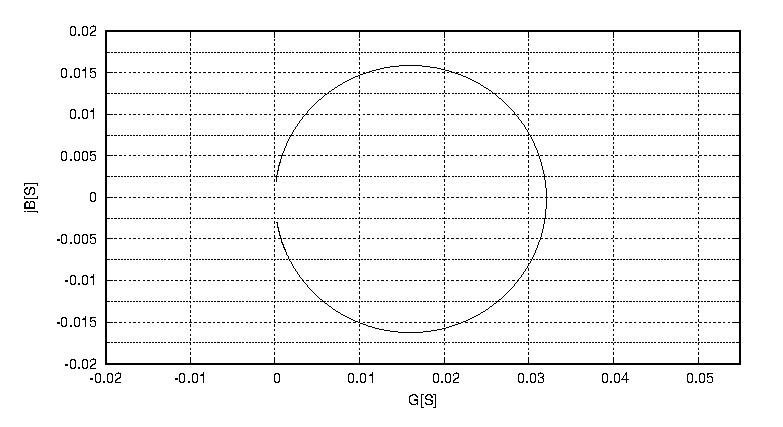
\includegraphics[width=10cm]{../gnuplot/A_GB.eps}
  \caption{R-L-C共振回路のアドミッタンスループ}
  \label{fig:A_GB.eps}
\end{figure}

\subsubsection{定数の算出}

\subsubsection{グラフの追記}

\section{課題}

\subsubsection{エミッタ接地,ベース接地,コレクタ接地の各増幅回路の特徴についてまとめよ.}

\subsubsection{共振回路の応用用途にはどのようなものがあるか調査し,それぞれについてまとめよ.}

\section{感想}

\begin{thebibliography}{99}
  \bibitem{umeda} 梅田 幹雄、実験テキスト「トランジスタの増幅回路とR-L-C共振回路」、(2022年)
  \bibitem{toshiba} 東芝トランジスタ、データシート「2SC1815」、(2017年11月1日)
\end{thebibliography}

\end{document}